\begin{figure}[H]
\centering
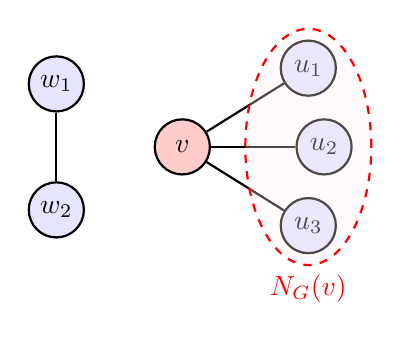
\begin{tikzpicture}[
  vnode/.style={circle, draw, minimum size=7mm, inner sep=0pt, fill=blue!10},
  thick
]
  \node[vnode, fill=red!20] (v) at (0, 0) {$v$};
  
  \node[vnode] (u1) at (1.6, 1) {$u_1$};
  \node[vnode] (u2) at (1.8, 0) {$u_2$};
  \node[vnode] (u3) at (1.6, -1) {$u_3$};
  
  \node[vnode] (w1) at (-1.6, 0.8) {$w_1$};
  \node[vnode] (w2) at (-1.6, -0.8) {$w_2$};
  
  \draw (v) -- (u1);
  \draw (v) -- (u2);
  \draw (v) -- (u3);
  \draw (w1) -- (w2);
  
  \draw[red, dashed, thick, fill=red!5, fill opacity=0.3] (1.6, 0) ellipse [x radius=0.8, y radius=1.5];
  \node[red] at (1.6, -1.8) {$N_G(v)$};
\end{tikzpicture}
\caption{Okolí $N_G(v)$ vrcholu $v$. Vrcholy $w_1$ and $w_2$ nepatří do okolí $v$.}
\end{figure}